\documentclass{article}
\usepackage[margin=2.2cm]{geometry}
\usepackage{booktabs}
\usepackage{array}
\usepackage{longtable}
\usepackage{float}
\usepackage[table]{xcolor}
\usepackage{hyperref}
\usepackage[utf8]{inputenc}
\usepackage{tikz}
\newcommand{\INF}{$\infty$}
\begin{document}
\begin{titlepage}
  \centering
  \vfill
  {\Huge Proyecto 1 - Rutas Òptimas Algoritmo de Floyd}\par
  \vspace{1cm}
  {\Large Curso: Investigación de Operaciones}\par
  {\Large Semestre: II Semestre 2025}\par
  \vfill
  {\Large Autores: Fabian Bustos - Esteban Secaida}\par
  \vspace{1cm}
  {\large Fecha: \today}\par
  \vfill
\end{titlepage}

\section*{Algoritmo de Floyd}
El algoritmo de Floyd, también conocido como Floyd--Warshall, es un método para encontrar las distancias más cortas entre todos los pares de nodos en un grafo ponderado, dirigido o no dirigido. Funciona de manera iterativa, actualizando las distancias considerando cada nodo como un posible punto intermedio entre pares de nodos.

El algoritmo fue propuesto por Robert W. Floyd en 1962, quien contribuyó significativamente al campo de la informática teórica y la optimización de algoritmos de grafos. La esencia de su trabajo reside en su simplicidad y eficacia para grafos densos.

\section*{Problema: Grafo de rutas}
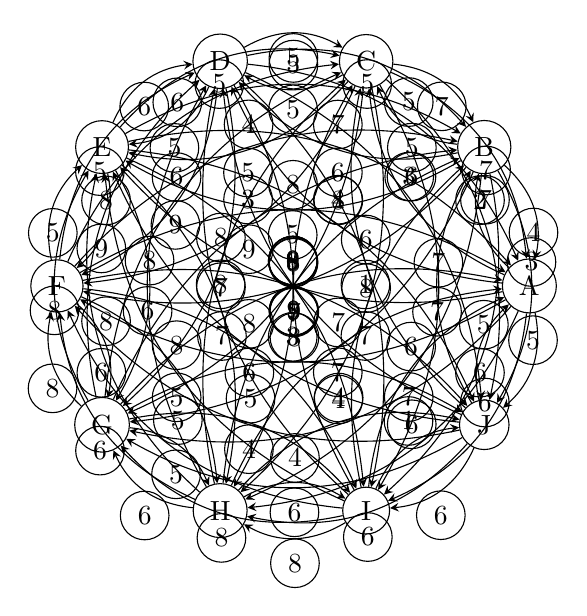
\begin{tikzpicture}[->, >=stealth, node distance=2cm, every node/.style={circle, draw}]
\node (0) at (0*360/10:3cm) {A};
\node (1) at (1*360/10:3cm) {B};
\node (2) at (2*360/10:3cm) {C};
\node (3) at (3*360/10:3cm) {D};
\node (4) at (4*360/10:3cm) {E};
\node (5) at (5*360/10:3cm) {F};
\node (6) at (6*360/10:3cm) {G};
\node (7) at (7*360/10:3cm) {H};
\node (8) at (8*360/10:3cm) {I};
\node (9) at (9*360/10:3cm) {J};
\draw (0) to[bend left] node[above] {2} (1);
\draw (1) to[bend left] node[below] {4} (0);
\draw (0) to[bend left] node[above] {3} (2);
\draw (2) to[bend left] node[below] {7} (0);
\draw (0) to[bend left] node[above] {4} (3);
\draw (3) to[bend left] node[below] {5} (0);
\draw (0) to[bend left] node[above] {3} (4);
\draw (4) to[bend left] node[below] {6} (0);
\draw (0) to[bend left] node[above] {3} (5);
\draw (5) to[bend left] node[below] {5} (0);
\draw (0) to[bend left] node[above] {4} (6);
\draw (6) to[bend left] node[below] {9} (0);
\draw (0) to[bend left] node[above] {6} (7);
\draw (7) to[bend left] node[below] {7} (0);
\draw (0) to[bend left] node[above] {6} (8);
\draw (8) to[bend left] node[below] {7} (0);
\draw (0) to[bend left] node[above] {5} (9);
\draw (9) to[bend left] node[below] {6} (0);
\draw (1) to[bend left] node[above] {5} (2);
\draw (2) to[bend left] node[below] {7} (1);
\draw (1) to[bend left] node[above] {7} (3);
\draw (3) to[bend left] node[below] {5} (1);
\draw (1) to[bend left] node[above] {8} (4);
\draw (4) to[bend left] node[below] {5} (1);
\draw (1) to[bend left] node[above] {9} (5);
\draw (5) to[bend left] node[below] {5} (1);
\draw (1) to[bend left] node[above] {7} (6);
\draw (6) to[bend left] node[below] {9} (1);
\draw (1) to[bend left] node[above] {6} (7);
\draw (7) to[bend left] node[below] {8} (1);
\draw (1) to[bend left] node[above] {5} (8);
\draw (8) to[bend left] node[below] {7} (1);
\draw (1) to[bend left] node[above] {3} (9);
\draw (9) to[bend left] node[below] {7} (1);
\draw (2) to[bend left] node[above] {5} (3);
\draw (3) to[bend left] node[below] {5} (2);
\draw (2) to[bend left] node[above] {4} (4);
\draw (4) to[bend left] node[below] {5} (2);
\draw (2) to[bend left] node[above] {3} (5);
\draw (5) to[bend left] node[below] {5} (2);
\draw (2) to[bend left] node[above] {9} (6);
\draw (6) to[bend left] node[below] {9} (2);
\draw (2) to[bend left] node[above] {1} (7);
\draw (7) to[bend left] node[below] {7} (2);
\draw (2) to[bend left] node[above] {7} (8);
\draw (8) to[bend left] node[below] {7} (2);
\draw (2) to[bend left] node[above] {7} (9);
\draw (9) to[bend left] node[below] {8} (2);
\draw (3) to[bend left] node[above] {6} (4);
\draw (4) to[bend left] node[below] {6} (3);
\draw (3) to[bend left] node[above] {6} (5);
\draw (5) to[bend left] node[below] {5} (3);
\draw (3) to[bend left] node[above] {8} (6);
\draw (6) to[bend left] node[below] {9} (3);
\draw (3) to[bend left] node[above] {6} (7);
\draw (7) to[bend left] node[below] {6} (3);
\draw (3) to[bend left] node[above] {6} (8);
\draw (8) to[bend left] node[below] {7} (3);
\draw (3) to[bend left] node[above] {6} (9);
\draw (9) to[bend left] node[below] {9} (3);
\draw (4) to[bend left] node[above] {8} (5);
\draw (5) to[bend left] node[below] {5} (4);
\draw (4) to[bend left] node[above] {8} (6);
\draw (6) to[bend left] node[below] {8} (4);
\draw (4) to[bend left] node[above] {8} (7);
\draw (7) to[bend left] node[below] {6} (4);
\draw (4) to[bend left] node[above] {8} (8);
\draw (8) to[bend left] node[below] {5} (4);
\draw (4) to[bend left] node[above] {8} (9);
\draw (9) to[bend left] node[below] {6} (4);
\draw (5) to[bend left] node[above] {8} (6);
\draw (6) to[bend left] node[below] {8} (5);
\draw (5) to[bend left] node[above] {8} (7);
\draw (7) to[bend left] node[below] {6} (5);
\draw (5) to[bend left] node[above] {8} (8);
\draw (8) to[bend left] node[below] {5} (5);
\draw (5) to[bend left] node[above] {8} (9);
\draw (9) to[bend left] node[below] {4} (5);
\draw (6) to[bend left] node[above] {5} (7);
\draw (7) to[bend left] node[below] {6} (6);
\draw (6) to[bend left] node[above] {5} (8);
\draw (8) to[bend left] node[below] {8} (6);
\draw (6) to[bend left] node[above] {8} (9);
\draw (9) to[bend left] node[below] {6} (6);
\draw (7) to[bend left] node[above] {4} (8);
\draw (8) to[bend left] node[below] {8} (7);
\draw (7) to[bend left] node[above] {4} (9);
\draw (9) to[bend left] node[below] {6} (7);
\draw (8) to[bend left] node[above] {1} (9);
\draw (9) to[bend left] node[below] {6} (8);
\end{tikzpicture}
\section*{Tablas Iniciales}
Reporte automático del algoritmo de Floyd--Warshall. Se muestran D(0) y P(0), todas las tablas intermedias D(k) y P(k) con cambios resaltados, y el resultado final.

\begin{table}[H]\centering
\caption{D(0) -- matriz de distancias inicial}
\rowcolors{2}{white}{white}
\begin{tabular}{l r r r r r r r r r r}
\toprule
 & \textbf{A} & \textbf{B} & \textbf{C} & \textbf{D} & \textbf{E} & \textbf{F} & \textbf{G} & \textbf{H} & \textbf{I} & \textbf{J}\\\midrule
\textbf{A} & 0 & 2 & 3 & 4 & 3 & 3 & 4 & 6 & 6 & 5 \\
\textbf{B} & 4 & 0 & 5 & 7 & 8 & 9 & 7 & 6 & 5 & 3 \\
\textbf{C} & 7 & 7 & 0 & 5 & 4 & 3 & 9 & 1 & 7 & 7 \\
\textbf{D} & 5 & 5 & 5 & 0 & 6 & 6 & 8 & 6 & 6 & 6 \\
\textbf{E} & 6 & 5 & 5 & 6 & 0 & 8 & 8 & 8 & 8 & 8 \\
\textbf{F} & 5 & 5 & 5 & 5 & 5 & 0 & 8 & 8 & 8 & 8 \\
\textbf{G} & 9 & 9 & 9 & 9 & 8 & 8 & 0 & 5 & 5 & 8 \\
\textbf{H} & 7 & 8 & 7 & 6 & 6 & 6 & 6 & 0 & 4 & 4 \\
\textbf{I} & 7 & 7 & 7 & 7 & 5 & 5 & 8 & 8 & 0 & 1 \\
\textbf{J} & 6 & 7 & 8 & 9 & 6 & 4 & 6 & 6 & 6 & 0 \\
\bottomrule
\end{tabular}
\end{table}

\begin{table}[H]\centering
\caption{P(0) -- matriz de siguiente salto inicial}
\rowcolors{2}{white}{white}
\begin{tabular}{l c c c c c c c c c c}
\toprule
 & \textbf{A} & \textbf{B} & \textbf{C} & \textbf{D} & \textbf{E} & \textbf{F} & \textbf{G} & \textbf{H} & \textbf{I} & \textbf{J}\\\midrule
\textbf{A} & - & B & C & D & E & F & G & H & I & J \\
\textbf{B} & A & - & C & D & E & F & G & H & I & J \\
\textbf{C} & A & B & - & D & E & F & G & H & I & J \\
\textbf{D} & A & B & C & - & E & F & G & H & I & J \\
\textbf{E} & A & B & C & D & - & F & G & H & I & J \\
\textbf{F} & A & B & C & D & E & - & G & H & I & J \\
\textbf{G} & A & B & C & D & E & F & - & H & I & J \\
\textbf{H} & A & B & C & D & E & F & G & - & I & J \\
\textbf{I} & A & B & C & D & E & F & G & H & - & J \\
\textbf{J} & A & B & C & D & E & F & G & H & I & - \\
\bottomrule
\end{tabular}
\end{table}

\section*{Tablas Intermedias}
\begin{table}[H]\centering
\caption{D(1)}
\rowcolors{2}{white}{white}
\begin{tabular}{l r r r r r r r r r r}
\toprule
 & \textbf{A} & \textbf{B} & \textbf{C} & \textbf{D} & \textbf{E} & \textbf{F} & \textbf{G} & \textbf{H} & \textbf{I} & \textbf{J}\\\midrule
\textbf{A} & 0 & 2 & 3 & 4 & 3 & 3 & 4 & 6 & 6 & 5 \\
\textbf{B} & 4 & 0 & 5 & 7 & \cellcolor{yellow!30}7 & \cellcolor{yellow!30}7 & 7 & 6 & 5 & 3 \\
\textbf{C} & 7 & 7 & 0 & 5 & 4 & 3 & 9 & 1 & 7 & 7 \\
\textbf{D} & 5 & 5 & 5 & 0 & 6 & 6 & 8 & 6 & 6 & 6 \\
\textbf{E} & 6 & 5 & 5 & 6 & 0 & 8 & 8 & 8 & 8 & 8 \\
\textbf{F} & 5 & 5 & 5 & 5 & 5 & 0 & 8 & 8 & 8 & 8 \\
\textbf{G} & 9 & 9 & 9 & 9 & 8 & 8 & 0 & 5 & 5 & 8 \\
\textbf{H} & 7 & 8 & 7 & 6 & 6 & 6 & 6 & 0 & 4 & 4 \\
\textbf{I} & 7 & 7 & 7 & 7 & 5 & 5 & 8 & 8 & 0 & 1 \\
\textbf{J} & 6 & 7 & 8 & 9 & 6 & 4 & 6 & 6 & 6 & 0 \\
\bottomrule
\end{tabular}
\end{table}

\begin{table}[H]\centering
\caption{P(1)}
\rowcolors{2}{white}{white}
\begin{tabular}{l c c c c c c c c c c}
\toprule
 & \textbf{A} & \textbf{B} & \textbf{C} & \textbf{D} & \textbf{E} & \textbf{F} & \textbf{G} & \textbf{H} & \textbf{I} & \textbf{J}\\\midrule
\textbf{A} & \cellcolor{yellow!30}A & B & C & D & E & F & G & H & I & J \\
\textbf{B} & A & \cellcolor{yellow!30}A & C & D & E & F & G & H & I & J \\
\textbf{C} & A & B & \cellcolor{yellow!30}A & D & E & F & G & H & I & J \\
\textbf{D} & A & B & C & \cellcolor{yellow!30}A & E & F & G & H & I & J \\
\textbf{E} & A & B & C & D & \cellcolor{yellow!30}A & F & G & H & I & J \\
\textbf{F} & A & B & C & D & E & \cellcolor{yellow!30}A & G & H & I & J \\
\textbf{G} & A & B & C & D & E & F & \cellcolor{yellow!30}A & H & I & J \\
\textbf{H} & A & B & C & D & E & F & G & \cellcolor{yellow!30}A & I & J \\
\textbf{I} & A & B & C & D & E & F & G & H & \cellcolor{yellow!30}A & J \\
\textbf{J} & A & B & C & D & E & F & G & H & I & \cellcolor{yellow!30}A \\
\bottomrule
\end{tabular}
\end{table}

\begin{table}[H]\centering
\caption{D(2)}
\rowcolors{2}{white}{white}
\begin{tabular}{l r r r r r r r r r r}
\toprule
 & \textbf{A} & \textbf{B} & \textbf{C} & \textbf{D} & \textbf{E} & \textbf{F} & \textbf{G} & \textbf{H} & \textbf{I} & \textbf{J}\\\midrule
\textbf{A} & 0 & 2 & 3 & 4 & 3 & 3 & 4 & 6 & 6 & 5 \\
\textbf{B} & 4 & 0 & 5 & 7 & 7 & 7 & 7 & 6 & 5 & 3 \\
\textbf{C} & 7 & 7 & 0 & 5 & 4 & 3 & 9 & 1 & 7 & 7 \\
\textbf{D} & 5 & 5 & 5 & 0 & 6 & 6 & 8 & 6 & 6 & 6 \\
\textbf{E} & 6 & 5 & 5 & 6 & 0 & 8 & 8 & 8 & 8 & 8 \\
\textbf{F} & 5 & 5 & 5 & 5 & 5 & 0 & 8 & 8 & 8 & 8 \\
\textbf{G} & 9 & 9 & 9 & 9 & 8 & 8 & 0 & 5 & 5 & 8 \\
\textbf{H} & 7 & 8 & 7 & 6 & 6 & 6 & 6 & 0 & 4 & 4 \\
\textbf{I} & 7 & 7 & 7 & 7 & 5 & 5 & 8 & 8 & 0 & 1 \\
\textbf{J} & 6 & 7 & 8 & 9 & 6 & 4 & 6 & 6 & 6 & 0 \\
\bottomrule
\end{tabular}
\end{table}

\begin{table}[H]\centering
\caption{P(2)}
\rowcolors{2}{white}{white}
\begin{tabular}{l c c c c c c c c c c}
\toprule
 & \textbf{A} & \textbf{B} & \textbf{C} & \textbf{D} & \textbf{E} & \textbf{F} & \textbf{G} & \textbf{H} & \textbf{I} & \textbf{J}\\\midrule
\textbf{A} & A & B & C & D & E & F & G & H & I & J \\
\textbf{B} & A & A & C & D & E & F & G & H & I & J \\
\textbf{C} & A & B & A & D & E & F & G & H & I & J \\
\textbf{D} & A & B & C & A & E & F & G & H & I & J \\
\textbf{E} & A & B & C & D & A & F & G & H & I & J \\
\textbf{F} & A & B & C & D & E & A & G & H & I & J \\
\textbf{G} & A & B & C & D & E & F & A & H & I & J \\
\textbf{H} & A & B & C & D & E & F & G & A & I & J \\
\textbf{I} & A & B & C & D & E & F & G & H & A & J \\
\textbf{J} & A & B & C & D & E & F & G & H & I & A \\
\bottomrule
\end{tabular}
\end{table}

\begin{table}[H]\centering
\caption{D(3)}
\rowcolors{2}{white}{white}
\begin{tabular}{l r r r r r r r r r r}
\toprule
 & \textbf{A} & \textbf{B} & \textbf{C} & \textbf{D} & \textbf{E} & \textbf{F} & \textbf{G} & \textbf{H} & \textbf{I} & \textbf{J}\\\midrule
\textbf{A} & 0 & 2 & 3 & 4 & 3 & 3 & 4 & \cellcolor{yellow!30}4 & 6 & 5 \\
\textbf{B} & 4 & 0 & 5 & 7 & 7 & 7 & 7 & 6 & 5 & 3 \\
\textbf{C} & 7 & 7 & 0 & 5 & 4 & 3 & 9 & 1 & 7 & 7 \\
\textbf{D} & 5 & 5 & 5 & 0 & 6 & 6 & 8 & 6 & 6 & 6 \\
\textbf{E} & 6 & 5 & 5 & 6 & 0 & 8 & 8 & \cellcolor{yellow!30}6 & 8 & 8 \\
\textbf{F} & 5 & 5 & 5 & 5 & 5 & 0 & 8 & \cellcolor{yellow!30}6 & 8 & 8 \\
\textbf{G} & 9 & 9 & 9 & 9 & 8 & 8 & 0 & 5 & 5 & 8 \\
\textbf{H} & 7 & 8 & 7 & 6 & 6 & 6 & 6 & 0 & 4 & 4 \\
\textbf{I} & 7 & 7 & 7 & 7 & 5 & 5 & 8 & 8 & 0 & 1 \\
\textbf{J} & 6 & 7 & 8 & 9 & 6 & 4 & 6 & 6 & 6 & 0 \\
\bottomrule
\end{tabular}
\end{table}

\begin{table}[H]\centering
\caption{P(3)}
\rowcolors{2}{white}{white}
\begin{tabular}{l c c c c c c c c c c}
\toprule
 & \textbf{A} & \textbf{B} & \textbf{C} & \textbf{D} & \textbf{E} & \textbf{F} & \textbf{G} & \textbf{H} & \textbf{I} & \textbf{J}\\\midrule
\textbf{A} & A & B & C & D & E & F & G & \cellcolor{yellow!30}C & I & J \\
\textbf{B} & A & A & C & D & E & F & G & H & I & J \\
\textbf{C} & A & B & A & D & E & F & G & H & I & J \\
\textbf{D} & A & B & C & A & E & F & G & H & I & J \\
\textbf{E} & A & B & C & D & A & F & G & \cellcolor{yellow!30}C & I & J \\
\textbf{F} & A & B & C & D & E & A & G & \cellcolor{yellow!30}C & I & J \\
\textbf{G} & A & B & C & D & E & F & A & H & I & J \\
\textbf{H} & A & B & C & D & E & F & G & A & I & J \\
\textbf{I} & A & B & C & D & E & F & G & H & A & J \\
\textbf{J} & A & B & C & D & E & F & G & H & I & A \\
\bottomrule
\end{tabular}
\end{table}

\begin{table}[H]\centering
\caption{D(4)}
\rowcolors{2}{white}{white}
\begin{tabular}{l r r r r r r r r r r}
\toprule
 & \textbf{A} & \textbf{B} & \textbf{C} & \textbf{D} & \textbf{E} & \textbf{F} & \textbf{G} & \textbf{H} & \textbf{I} & \textbf{J}\\\midrule
\textbf{A} & 0 & 2 & 3 & 4 & 3 & 3 & 4 & 4 & 6 & 5 \\
\textbf{B} & 4 & 0 & 5 & 7 & 7 & 7 & 7 & 6 & 5 & 3 \\
\textbf{C} & 7 & 7 & 0 & 5 & 4 & 3 & 9 & 1 & 7 & 7 \\
\textbf{D} & 5 & 5 & 5 & 0 & 6 & 6 & 8 & 6 & 6 & 6 \\
\textbf{E} & 6 & 5 & 5 & 6 & 0 & 8 & 8 & 6 & 8 & 8 \\
\textbf{F} & 5 & 5 & 5 & 5 & 5 & 0 & 8 & 6 & 8 & 8 \\
\textbf{G} & 9 & 9 & 9 & 9 & 8 & 8 & 0 & 5 & 5 & 8 \\
\textbf{H} & 7 & 8 & 7 & 6 & 6 & 6 & 6 & 0 & 4 & 4 \\
\textbf{I} & 7 & 7 & 7 & 7 & 5 & 5 & 8 & 8 & 0 & 1 \\
\textbf{J} & 6 & 7 & 8 & 9 & 6 & 4 & 6 & 6 & 6 & 0 \\
\bottomrule
\end{tabular}
\end{table}

\begin{table}[H]\centering
\caption{P(4)}
\rowcolors{2}{white}{white}
\begin{tabular}{l c c c c c c c c c c}
\toprule
 & \textbf{A} & \textbf{B} & \textbf{C} & \textbf{D} & \textbf{E} & \textbf{F} & \textbf{G} & \textbf{H} & \textbf{I} & \textbf{J}\\\midrule
\textbf{A} & A & B & C & D & E & F & G & C & I & J \\
\textbf{B} & A & A & C & D & E & F & G & H & I & J \\
\textbf{C} & A & B & A & D & E & F & G & H & I & J \\
\textbf{D} & A & B & C & A & E & F & G & H & I & J \\
\textbf{E} & A & B & C & D & A & F & G & C & I & J \\
\textbf{F} & A & B & C & D & E & A & G & C & I & J \\
\textbf{G} & A & B & C & D & E & F & A & H & I & J \\
\textbf{H} & A & B & C & D & E & F & G & A & I & J \\
\textbf{I} & A & B & C & D & E & F & G & H & A & J \\
\textbf{J} & A & B & C & D & E & F & G & H & I & A \\
\bottomrule
\end{tabular}
\end{table}

\begin{table}[H]\centering
\caption{D(5)}
\rowcolors{2}{white}{white}
\begin{tabular}{l r r r r r r r r r r}
\toprule
 & \textbf{A} & \textbf{B} & \textbf{C} & \textbf{D} & \textbf{E} & \textbf{F} & \textbf{G} & \textbf{H} & \textbf{I} & \textbf{J}\\\midrule
\textbf{A} & 0 & 2 & 3 & 4 & 3 & 3 & 4 & 4 & 6 & 5 \\
\textbf{B} & 4 & 0 & 5 & 7 & 7 & 7 & 7 & 6 & 5 & 3 \\
\textbf{C} & 7 & 7 & 0 & 5 & 4 & 3 & 9 & 1 & 7 & 7 \\
\textbf{D} & 5 & 5 & 5 & 0 & 6 & 6 & 8 & 6 & 6 & 6 \\
\textbf{E} & 6 & 5 & 5 & 6 & 0 & 8 & 8 & 6 & 8 & 8 \\
\textbf{F} & 5 & 5 & 5 & 5 & 5 & 0 & 8 & 6 & 8 & 8 \\
\textbf{G} & 9 & 9 & 9 & 9 & 8 & 8 & 0 & 5 & 5 & 8 \\
\textbf{H} & 7 & 8 & 7 & 6 & 6 & 6 & 6 & 0 & 4 & 4 \\
\textbf{I} & 7 & 7 & 7 & 7 & 5 & 5 & 8 & 8 & 0 & 1 \\
\textbf{J} & 6 & 7 & 8 & 9 & 6 & 4 & 6 & 6 & 6 & 0 \\
\bottomrule
\end{tabular}
\end{table}

\begin{table}[H]\centering
\caption{P(5)}
\rowcolors{2}{white}{white}
\begin{tabular}{l c c c c c c c c c c}
\toprule
 & \textbf{A} & \textbf{B} & \textbf{C} & \textbf{D} & \textbf{E} & \textbf{F} & \textbf{G} & \textbf{H} & \textbf{I} & \textbf{J}\\\midrule
\textbf{A} & A & B & C & D & E & F & G & C & I & J \\
\textbf{B} & A & A & C & D & E & F & G & H & I & J \\
\textbf{C} & A & B & A & D & E & F & G & H & I & J \\
\textbf{D} & A & B & C & A & E & F & G & H & I & J \\
\textbf{E} & A & B & C & D & A & F & G & C & I & J \\
\textbf{F} & A & B & C & D & E & A & G & C & I & J \\
\textbf{G} & A & B & C & D & E & F & A & H & I & J \\
\textbf{H} & A & B & C & D & E & F & G & A & I & J \\
\textbf{I} & A & B & C & D & E & F & G & H & A & J \\
\textbf{J} & A & B & C & D & E & F & G & H & I & A \\
\bottomrule
\end{tabular}
\end{table}

\begin{table}[H]\centering
\caption{D(6)}
\rowcolors{2}{white}{white}
\begin{tabular}{l r r r r r r r r r r}
\toprule
 & \textbf{A} & \textbf{B} & \textbf{C} & \textbf{D} & \textbf{E} & \textbf{F} & \textbf{G} & \textbf{H} & \textbf{I} & \textbf{J}\\\midrule
\textbf{A} & 0 & 2 & 3 & 4 & 3 & 3 & 4 & 4 & 6 & 5 \\
\textbf{B} & 4 & 0 & 5 & 7 & 7 & 7 & 7 & 6 & 5 & 3 \\
\textbf{C} & 7 & 7 & 0 & 5 & 4 & 3 & 9 & 1 & 7 & 7 \\
\textbf{D} & 5 & 5 & 5 & 0 & 6 & 6 & 8 & 6 & 6 & 6 \\
\textbf{E} & 6 & 5 & 5 & 6 & 0 & 8 & 8 & 6 & 8 & 8 \\
\textbf{F} & 5 & 5 & 5 & 5 & 5 & 0 & 8 & 6 & 8 & 8 \\
\textbf{G} & 9 & 9 & 9 & 9 & 8 & 8 & 0 & 5 & 5 & 8 \\
\textbf{H} & 7 & 8 & 7 & 6 & 6 & 6 & 6 & 0 & 4 & 4 \\
\textbf{I} & 7 & 7 & 7 & 7 & 5 & 5 & 8 & 8 & 0 & 1 \\
\textbf{J} & 6 & 7 & 8 & 9 & 6 & 4 & 6 & 6 & 6 & 0 \\
\bottomrule
\end{tabular}
\end{table}

\begin{table}[H]\centering
\caption{P(6)}
\rowcolors{2}{white}{white}
\begin{tabular}{l c c c c c c c c c c}
\toprule
 & \textbf{A} & \textbf{B} & \textbf{C} & \textbf{D} & \textbf{E} & \textbf{F} & \textbf{G} & \textbf{H} & \textbf{I} & \textbf{J}\\\midrule
\textbf{A} & A & B & C & D & E & F & G & C & I & J \\
\textbf{B} & A & A & C & D & E & F & G & H & I & J \\
\textbf{C} & A & B & A & D & E & F & G & H & I & J \\
\textbf{D} & A & B & C & A & E & F & G & H & I & J \\
\textbf{E} & A & B & C & D & A & F & G & C & I & J \\
\textbf{F} & A & B & C & D & E & A & G & C & I & J \\
\textbf{G} & A & B & C & D & E & F & A & H & I & J \\
\textbf{H} & A & B & C & D & E & F & G & A & I & J \\
\textbf{I} & A & B & C & D & E & F & G & H & A & J \\
\textbf{J} & A & B & C & D & E & F & G & H & I & A \\
\bottomrule
\end{tabular}
\end{table}

\begin{table}[H]\centering
\caption{D(7)}
\rowcolors{2}{white}{white}
\begin{tabular}{l r r r r r r r r r r}
\toprule
 & \textbf{A} & \textbf{B} & \textbf{C} & \textbf{D} & \textbf{E} & \textbf{F} & \textbf{G} & \textbf{H} & \textbf{I} & \textbf{J}\\\midrule
\textbf{A} & 0 & 2 & 3 & 4 & 3 & 3 & 4 & 4 & 6 & 5 \\
\textbf{B} & 4 & 0 & 5 & 7 & 7 & 7 & 7 & 6 & 5 & 3 \\
\textbf{C} & 7 & 7 & 0 & 5 & 4 & 3 & 9 & 1 & 7 & 7 \\
\textbf{D} & 5 & 5 & 5 & 0 & 6 & 6 & 8 & 6 & 6 & 6 \\
\textbf{E} & 6 & 5 & 5 & 6 & 0 & 8 & 8 & 6 & 8 & 8 \\
\textbf{F} & 5 & 5 & 5 & 5 & 5 & 0 & 8 & 6 & 8 & 8 \\
\textbf{G} & 9 & 9 & 9 & 9 & 8 & 8 & 0 & 5 & 5 & 8 \\
\textbf{H} & 7 & 8 & 7 & 6 & 6 & 6 & 6 & 0 & 4 & 4 \\
\textbf{I} & 7 & 7 & 7 & 7 & 5 & 5 & 8 & 8 & 0 & 1 \\
\textbf{J} & 6 & 7 & 8 & 9 & 6 & 4 & 6 & 6 & 6 & 0 \\
\bottomrule
\end{tabular}
\end{table}

\begin{table}[H]\centering
\caption{P(7)}
\rowcolors{2}{white}{white}
\begin{tabular}{l c c c c c c c c c c}
\toprule
 & \textbf{A} & \textbf{B} & \textbf{C} & \textbf{D} & \textbf{E} & \textbf{F} & \textbf{G} & \textbf{H} & \textbf{I} & \textbf{J}\\\midrule
\textbf{A} & A & B & C & D & E & F & G & C & I & J \\
\textbf{B} & A & A & C & D & E & F & G & H & I & J \\
\textbf{C} & A & B & A & D & E & F & G & H & I & J \\
\textbf{D} & A & B & C & A & E & F & G & H & I & J \\
\textbf{E} & A & B & C & D & A & F & G & C & I & J \\
\textbf{F} & A & B & C & D & E & A & G & C & I & J \\
\textbf{G} & A & B & C & D & E & F & A & H & I & J \\
\textbf{H} & A & B & C & D & E & F & G & A & I & J \\
\textbf{I} & A & B & C & D & E & F & G & H & A & J \\
\textbf{J} & A & B & C & D & E & F & G & H & I & A \\
\bottomrule
\end{tabular}
\end{table}

\begin{table}[H]\centering
\caption{D(8)}
\rowcolors{2}{white}{white}
\begin{tabular}{l r r r r r r r r r r}
\toprule
 & \textbf{A} & \textbf{B} & \textbf{C} & \textbf{D} & \textbf{E} & \textbf{F} & \textbf{G} & \textbf{H} & \textbf{I} & \textbf{J}\\\midrule
\textbf{A} & 0 & 2 & 3 & 4 & 3 & 3 & 4 & 4 & 6 & 5 \\
\textbf{B} & 4 & 0 & 5 & 7 & 7 & 7 & 7 & 6 & 5 & 3 \\
\textbf{C} & 7 & 7 & 0 & 5 & 4 & 3 & \cellcolor{yellow!30}7 & 1 & \cellcolor{yellow!30}5 & \cellcolor{yellow!30}5 \\
\textbf{D} & 5 & 5 & 5 & 0 & 6 & 6 & 8 & 6 & 6 & 6 \\
\textbf{E} & 6 & 5 & 5 & 6 & 0 & 8 & 8 & 6 & 8 & 8 \\
\textbf{F} & 5 & 5 & 5 & 5 & 5 & 0 & 8 & 6 & 8 & 8 \\
\textbf{G} & 9 & 9 & 9 & 9 & 8 & 8 & 0 & 5 & 5 & 8 \\
\textbf{H} & 7 & 8 & 7 & 6 & 6 & 6 & 6 & 0 & 4 & 4 \\
\textbf{I} & 7 & 7 & 7 & 7 & 5 & 5 & 8 & 8 & 0 & 1 \\
\textbf{J} & 6 & 7 & 8 & 9 & 6 & 4 & 6 & 6 & 6 & 0 \\
\bottomrule
\end{tabular}
\end{table}

\begin{table}[H]\centering
\caption{P(8)}
\rowcolors{2}{white}{white}
\begin{tabular}{l c c c c c c c c c c}
\toprule
 & \textbf{A} & \textbf{B} & \textbf{C} & \textbf{D} & \textbf{E} & \textbf{F} & \textbf{G} & \textbf{H} & \textbf{I} & \textbf{J}\\\midrule
\textbf{A} & A & B & C & D & E & F & G & C & I & J \\
\textbf{B} & A & A & C & D & E & F & G & H & I & J \\
\textbf{C} & A & B & A & D & E & F & \cellcolor{yellow!30}H & H & \cellcolor{yellow!30}H & \cellcolor{yellow!30}H \\
\textbf{D} & A & B & C & A & E & F & G & H & I & J \\
\textbf{E} & A & B & C & D & A & F & G & C & I & J \\
\textbf{F} & A & B & C & D & E & A & G & C & I & J \\
\textbf{G} & A & B & C & D & E & F & A & H & I & J \\
\textbf{H} & A & B & C & D & E & F & G & A & I & J \\
\textbf{I} & A & B & C & D & E & F & G & H & A & J \\
\textbf{J} & A & B & C & D & E & F & G & H & I & A \\
\bottomrule
\end{tabular}
\end{table}

\begin{table}[H]\centering
\caption{D(9)}
\rowcolors{2}{white}{white}
\begin{tabular}{l r r r r r r r r r r}
\toprule
 & \textbf{A} & \textbf{B} & \textbf{C} & \textbf{D} & \textbf{E} & \textbf{F} & \textbf{G} & \textbf{H} & \textbf{I} & \textbf{J}\\\midrule
\textbf{A} & 0 & 2 & 3 & 4 & 3 & 3 & 4 & 4 & 6 & 5 \\
\textbf{B} & 4 & 0 & 5 & 7 & 7 & 7 & 7 & 6 & 5 & 3 \\
\textbf{C} & 7 & 7 & 0 & 5 & 4 & 3 & 7 & 1 & 5 & 5 \\
\textbf{D} & 5 & 5 & 5 & 0 & 6 & 6 & 8 & 6 & 6 & 6 \\
\textbf{E} & 6 & 5 & 5 & 6 & 0 & 8 & 8 & 6 & 8 & 8 \\
\textbf{F} & 5 & 5 & 5 & 5 & 5 & 0 & 8 & 6 & 8 & 8 \\
\textbf{G} & 9 & 9 & 9 & 9 & 8 & 8 & 0 & 5 & 5 & \cellcolor{yellow!30}6 \\
\textbf{H} & 7 & 8 & 7 & 6 & 6 & 6 & 6 & 0 & 4 & 4 \\
\textbf{I} & 7 & 7 & 7 & 7 & 5 & 5 & 8 & 8 & 0 & 1 \\
\textbf{J} & 6 & 7 & 8 & 9 & 6 & 4 & 6 & 6 & 6 & 0 \\
\bottomrule
\end{tabular}
\end{table}

\begin{table}[H]\centering
\caption{P(9)}
\rowcolors{2}{white}{white}
\begin{tabular}{l c c c c c c c c c c}
\toprule
 & \textbf{A} & \textbf{B} & \textbf{C} & \textbf{D} & \textbf{E} & \textbf{F} & \textbf{G} & \textbf{H} & \textbf{I} & \textbf{J}\\\midrule
\textbf{A} & A & B & C & D & E & F & G & C & I & J \\
\textbf{B} & A & A & C & D & E & F & G & H & I & J \\
\textbf{C} & A & B & A & D & E & F & H & H & H & H \\
\textbf{D} & A & B & C & A & E & F & G & H & I & J \\
\textbf{E} & A & B & C & D & A & F & G & C & I & J \\
\textbf{F} & A & B & C & D & E & A & G & C & I & J \\
\textbf{G} & A & B & C & D & E & F & A & H & I & \cellcolor{yellow!30}I \\
\textbf{H} & A & B & C & D & E & F & G & A & I & J \\
\textbf{I} & A & B & C & D & E & F & G & H & A & J \\
\textbf{J} & A & B & C & D & E & F & G & H & I & A \\
\bottomrule
\end{tabular}
\end{table}

\begin{table}[H]\centering
\caption{D(10)}
\rowcolors{2}{white}{white}
\begin{tabular}{l r r r r r r r r r r}
\toprule
 & \textbf{A} & \textbf{B} & \textbf{C} & \textbf{D} & \textbf{E} & \textbf{F} & \textbf{G} & \textbf{H} & \textbf{I} & \textbf{J}\\\midrule
\textbf{A} & 0 & 2 & 3 & 4 & 3 & 3 & 4 & 4 & 6 & 5 \\
\textbf{B} & 4 & 0 & 5 & 7 & 7 & 7 & 7 & 6 & 5 & 3 \\
\textbf{C} & 7 & 7 & 0 & 5 & 4 & 3 & 7 & 1 & 5 & 5 \\
\textbf{D} & 5 & 5 & 5 & 0 & 6 & 6 & 8 & 6 & 6 & 6 \\
\textbf{E} & 6 & 5 & 5 & 6 & 0 & 8 & 8 & 6 & 8 & 8 \\
\textbf{F} & 5 & 5 & 5 & 5 & 5 & 0 & 8 & 6 & 8 & 8 \\
\textbf{G} & 9 & 9 & 9 & 9 & 8 & 8 & 0 & 5 & 5 & 6 \\
\textbf{H} & 7 & 8 & 7 & 6 & 6 & 6 & 6 & 0 & 4 & 4 \\
\textbf{I} & 7 & 7 & 7 & 7 & 5 & 5 & \cellcolor{yellow!30}7 & \cellcolor{yellow!30}7 & 0 & 1 \\
\textbf{J} & 6 & 7 & 8 & 9 & 6 & 4 & 6 & 6 & 6 & 0 \\
\bottomrule
\end{tabular}
\end{table}

\begin{table}[H]\centering
\caption{P(10)}
\rowcolors{2}{white}{white}
\begin{tabular}{l c c c c c c c c c c}
\toprule
 & \textbf{A} & \textbf{B} & \textbf{C} & \textbf{D} & \textbf{E} & \textbf{F} & \textbf{G} & \textbf{H} & \textbf{I} & \textbf{J}\\\midrule
\textbf{A} & A & B & C & D & E & F & G & C & I & J \\
\textbf{B} & A & A & C & D & E & F & G & H & I & J \\
\textbf{C} & A & B & A & D & E & F & H & H & H & H \\
\textbf{D} & A & B & C & A & E & F & G & H & I & J \\
\textbf{E} & A & B & C & D & A & F & G & C & I & J \\
\textbf{F} & A & B & C & D & E & A & G & C & I & J \\
\textbf{G} & A & B & C & D & E & F & A & H & I & I \\
\textbf{H} & A & B & C & D & E & F & G & A & I & J \\
\textbf{I} & A & B & C & D & E & F & \cellcolor{yellow!30}J & \cellcolor{yellow!30}J & A & J \\
\textbf{J} & A & B & C & D & E & F & G & H & I & A \\
\bottomrule
\end{tabular}
\end{table}

\section*{Distancias y rutas óptimas}
\begin{table}[H]\centering
\caption{D(final)}
\rowcolors{2}{white}{white}
\begin{tabular}{l r r r r r r r r r r}
\toprule
 & \textbf{A} & \textbf{B} & \textbf{C} & \textbf{D} & \textbf{E} & \textbf{F} & \textbf{G} & \textbf{H} & \textbf{I} & \textbf{J}\\\midrule
\textbf{A} & 0 & 2 & 3 & 4 & 3 & 3 & 4 & 4 & 6 & 5 \\
\textbf{B} & 4 & 0 & 5 & 7 & 7 & 7 & 7 & 6 & 5 & 3 \\
\textbf{C} & 7 & 7 & 0 & 5 & 4 & 3 & 7 & 1 & 5 & 5 \\
\textbf{D} & 5 & 5 & 5 & 0 & 6 & 6 & 8 & 6 & 6 & 6 \\
\textbf{E} & 6 & 5 & 5 & 6 & 0 & 8 & 8 & 6 & 8 & 8 \\
\textbf{F} & 5 & 5 & 5 & 5 & 5 & 0 & 8 & 6 & 8 & 8 \\
\textbf{G} & 9 & 9 & 9 & 9 & 8 & 8 & 0 & 5 & 5 & 6 \\
\textbf{H} & 7 & 8 & 7 & 6 & 6 & 6 & 6 & 0 & 4 & 4 \\
\textbf{I} & 7 & 7 & 7 & 7 & 5 & 5 & 7 & 7 & 0 & 1 \\
\textbf{J} & 6 & 7 & 8 & 9 & 6 & 4 & 6 & 6 & 6 & 0 \\
\bottomrule
\end{tabular}
\end{table}

\begin{table}[H]\centering
\caption{P(final)}
\rowcolors{2}{white}{white}
\begin{tabular}{l c c c c c c c c c c}
\toprule
 & \textbf{A} & \textbf{B} & \textbf{C} & \textbf{D} & \textbf{E} & \textbf{F} & \textbf{G} & \textbf{H} & \textbf{I} & \textbf{J}\\\midrule
\textbf{A} & A & B & C & D & E & F & G & C & I & J \\
\textbf{B} & A & A & C & D & E & F & G & H & I & J \\
\textbf{C} & A & B & A & D & E & F & H & H & H & H \\
\textbf{D} & A & B & C & A & E & F & G & H & I & J \\
\textbf{E} & A & B & C & D & A & F & G & C & I & J \\
\textbf{F} & A & B & C & D & E & A & G & C & I & J \\
\textbf{G} & A & B & C & D & E & F & A & H & I & I \\
\textbf{H} & A & B & C & D & E & F & G & A & I & J \\
\textbf{I} & A & B & C & D & E & F & J & J & A & J \\
\textbf{J} & A & B & C & D & E & F & G & H & I & A \\
\bottomrule
\end{tabular}
\end{table}

\subsection*{Listado de rutas (todas las parejas i $\neq$ j)}
\begin{longtable}{llp{0.65\textwidth}}
\toprule
\textbf{Origen} & \textbf{Destino} & \textbf{Ruta óptima (con saltos)}\\\midrule
A & B & A → B (distancia = 2)\\
A & C & A → C (distancia = 3)\\
A & D & A → D (distancia = 4)\\
A & E & A → E (distancia = 3)\\
A & F & A → F (distancia = 3)\\
A & G & A → G (distancia = 4)\\
A & H & A → C → H (distancia = 4)\\
A & I & A → I (distancia = 6)\\
A & J & A → J (distancia = 5)\\
B & A & B → A (distancia = 4)\\
B & C & B → C (distancia = 5)\\
B & D & B → D (distancia = 7)\\
B & E & B → E (distancia = 7)\\
B & F & B → F (distancia = 7)\\
B & G & B → G (distancia = 7)\\
B & H & B → H (distancia = 6)\\
B & I & B → I (distancia = 5)\\
B & J & B → J (distancia = 3)\\
C & A & C → A (distancia = 7)\\
C & B & C → B (distancia = 7)\\
C & D & C → D (distancia = 5)\\
C & E & C → E (distancia = 4)\\
C & F & C → F (distancia = 3)\\
C & G & C → H → G (distancia = 7)\\
C & H & C → H (distancia = 1)\\
C & I & C → H → I (distancia = 5)\\
C & J & C → H → J (distancia = 5)\\
D & A & D → A (distancia = 5)\\
D & B & D → B (distancia = 5)\\
D & C & D → C (distancia = 5)\\
D & E & D → E (distancia = 6)\\
D & F & D → F (distancia = 6)\\
D & G & D → G (distancia = 8)\\
D & H & D → H (distancia = 6)\\
D & I & D → I (distancia = 6)\\
D & J & D → J (distancia = 6)\\
E & A & E → A (distancia = 6)\\
E & B & E → B (distancia = 5)\\
E & C & E → C (distancia = 5)\\
E & D & E → D (distancia = 6)\\
E & F & E → F (distancia = 8)\\
E & G & E → G (distancia = 8)\\
E & H & E → C → H (distancia = 6)\\
E & I & E → I (distancia = 8)\\
E & J & E → J (distancia = 8)\\
F & A & F → A (distancia = 5)\\
F & B & F → B (distancia = 5)\\
F & C & F → C (distancia = 5)\\
F & D & F → D (distancia = 5)\\
F & E & F → E (distancia = 5)\\
F & G & F → G (distancia = 8)\\
F & H & F → C → H (distancia = 6)\\
F & I & F → I (distancia = 8)\\
F & J & F → J (distancia = 8)\\
G & A & G → A (distancia = 9)\\
G & B & G → B (distancia = 9)\\
G & C & G → C (distancia = 9)\\
G & D & G → D (distancia = 9)\\
G & E & G → E (distancia = 8)\\
G & F & G → F (distancia = 8)\\
G & H & G → H (distancia = 5)\\
G & I & G → I (distancia = 5)\\
G & J & G → I → J (distancia = 6)\\
H & A & H → A (distancia = 7)\\
H & B & H → B (distancia = 8)\\
H & C & H → C (distancia = 7)\\
H & D & H → D (distancia = 6)\\
H & E & H → E (distancia = 6)\\
H & F & H → F (distancia = 6)\\
H & G & H → G (distancia = 6)\\
H & I & H → I (distancia = 4)\\
H & J & H → J (distancia = 4)\\
I & A & I → A (distancia = 7)\\
I & B & I → B (distancia = 7)\\
I & C & I → C (distancia = 7)\\
I & D & I → D (distancia = 7)\\
I & E & I → E (distancia = 5)\\
I & F & I → F (distancia = 5)\\
I & G & I → J → G (distancia = 7)\\
I & H & I → J → H (distancia = 7)\\
I & J & I → J (distancia = 1)\\
J & A & J → A (distancia = 6)\\
J & B & J → B (distancia = 7)\\
J & C & J → C (distancia = 8)\\
J & D & J → D (distancia = 9)\\
J & E & J → E (distancia = 6)\\
J & F & J → F (distancia = 4)\\
J & G & J → G (distancia = 6)\\
J & H & J → H (distancia = 6)\\
J & I & J → I (distancia = 6)\\
\bottomrule
\end{longtable}
\end{document}